%\chapter[State of art]{\begin {Huge}\textit{\bf{State of art}} \end{Huge}}

\chapter[GNSS Raw Measurements and RTKLIB]{\centering \begin{normalsize} \begin{Huge}
		GNSS Raw Measurements and RTKLIB
\end{Huge} \end{normalsize}}
\label{ch:SoA}
%GNSS positioning 
%from Android devices  and 
%This chapter explains the basics of GNSS positioning from Android devices. After highlighting the main research in this area, the Android API that allows access to GNSS raw data in smartphones is explained in detail. The various quantities that can be accessed are then explained and how they can be used to reconstruct classical GNSS observables, i.e. pseudorange, carrier phase, doppler and Signal to Noise Ratio which is an indicator of the quality of the incoming signal. In the latter part of the chapter the GNSS processing software RTKLIB is described. (LB: Non mi convince molto come intro)      
%
\section{GNSS Positioning in Android}
Starting in 2016, with the Android Nougat 7.0 Operating System (OS) development, Google has permitted direct access to the GNSS chipset raw measurements mounted on some Android-based smartphones. The possibility to exploit smartphone GNSS integrated chipset started a new research field aimed at exploiting them in new low-cost applications for satellite-based positioning. 
Even before Google started providing open access to  raw data, the feasibility to perform GNSS positioning using low-cost receivers and smartphone antennas was investigated. In \cite{Pesyna2014} authors showed that centimetric accuracy could be achieved by using a smartphone quality GNSS antenna in relative positioning mode. They also demonstrated that the smartphone GNSS observations are highly affected by the multipath error. In fact, as explained in \cite{Humphreys:2016} the most critical issue is related to the employed GNSS  
 antenna. The smartphone antenna uses linear polarization with non homogeneous gain and high levels of local multipath which render the goal of achieving centimetric accuracy  significantly challenging. Many other researches have been conducted exploring the possibility of managing pseudo-range and carrier phase measurements from the GNSS chipset installed on Android OS smartphones and tablets. 
In a sense, Android OS has changed the concept of precise positioning with portable devices. In this setting different scenarios have been investigated, ranging from urban \cite{Masiero2014, wang2015, wang2016a, wang2016b, adjrad2018} applications  to pedestrian positioning  \cite{Fissore2018, presti2017}, always facing problems related to difficulties in the correct use of the Android Application Programming Interface (API) and of the corresponding filtered measurements provided by the GNSS chipset.

Thanks to the release of a white paper  of the European GNSS Agency \cite{GSA_wp:2016}, in which detailed guidelines on how to reconstruct GNSS measurements using the Android API are given, many authors started to analyze the quality of the raw measurements retrieved from smartphones. The main detected issues in most of the considered experiments were due to the duty cycle mechanism and to low values of the C/N\textsubscript{0} \cite{gogoi2019,Liu:2019} parameter.

In \cite{banville2016} authors conducted an investigation on the quality of the real raw GNSS observations from the smartphones with the purpose of high precision positioning. They analyzed the data collected by a Samsung Galaxy S7 smartphone equipped with the Broadcom 4774 GNSS chip which is able to log raw multi-GNSS (GPS, GLONASS, BDS, Galileo, and QZSS) observations on the L1 frequency. However, in their work, the authors only employed the GPS observations. Since the true position of the smartphone is unknown, they estimated the positioning errors for all components with respect to the mean values of each component. The results indicated that the pseudorange
observations are noisy and only capable of providing meter-level accuracy. They also mentioned that the carrier-phase observations from the smartphones can potentially provide an opportunity to achieve decimeter level or better positioning accuracy. However, to obtain high-accuracy positioning, some important issues such as the quality of the smartphone antenna and the GNSS
duty cycling, a battery saving mode for the GNSS chip causing discontinuities in carrier-phase observations, must be taken into account.
In \cite{Lachapelle2018}, instead, the authors compared the performance of a hand-held GNSS Garmin GPSMap 66 unit with a Huawei P10 smartphone under different conditions including on a rooftop of a building, an urban canyon, indoors and in a car. The results indicated a relatively better performance of the GPSMap 66 with respect to the Huawei P10 which is due to the lower gain advantage of the GPSMap 66 over the P10. It was also shown that the use of an external geodetic antenna can significantly improve data quality and positioning accuracy.
The quality of the raw smartphone observations was also investigated in \cite{Zhang:2018} and the authors draw the same conclusions as the other researchers about the relatively low quality of the smartphone GNSS observations. They also showed that C/N\textsubscript{0} value of GNSS raw observations of the smartphones is 10 dB-Hz lower than the C/N\textsubscript{0} values obtained from a geodetic-quality antenna and receiver. They then combined the pseudorange, carrier-phase and Doppler observations by a time-difference filter positioning algorithm. In this method, they used the Doppler observations to obtain the velocities and then combined them with the single point positioning solutions to achieve the sub-meter level positioning accuracy.
GNSS raw measurement from smartphone were also elaborated using different post-processing techniques. In \cite{Gill2018} authors assessed the accuracy of GPS-only single-frequency PPP with a Nexus 9 smartphone by employing the Global Ionospheric Maps (GIM) to account for the ionospheric delay. The results indicated the RMS of 37 cm and 51 cm for the horizontal and vertical components, respectively, using the cellphone. 
In \cite{realini2017}, the authors demonstrated that it was possible to reach  decimetric  accuracy in terms of positioning performances following the post-processing approach, via a double difference of raw smartphone observations. Meanwhile, the authors of \cite{Dabove2019b} first focused their attention on single-base RTK positioning and then demonstrated the possibility
of obtaining a centimeter-level accuracy through the use of NRTK corrections \cite{Dabove2019b}.
These results are supported by the authors in \cite{pirazzi2017}, who, employing a variometric approach, show decimeter accuracy in static condition and sub-meter when used in an urban vehicle scenario.

Another milestone has been set by Broadcom, announcing on September 21, 2017, the world’s first mass-market, dual-frequency GNSS receiver device, the BCM47755. In May 2018, the Xiaomi Mi8 became the first smartphone in the world, employing a dual-frequency
GNSS receiver L1/E1 – L5/E5a. This led to the next series of studies in the investigation of smartphone-based positioning. 
The NSL’s FLAMINGO (Nottingham Scientific Limited’s fulfilling enhanced location accuracy in the mass-market through Initial Galileo Services) team investigated the PPP and RTK performance of the dual-frequency Xiaomi Mi8 smartphone \cite{Fortunato2019,Roberts2018}. The results confirmed that the carrier-phase observations from the Xiaomi Mi8 were not affected by the duty cycling and employing the L5/E5a observations could improve the positioning accuracy.
Thanks to the double frequency introduced in \cite{Robustelli:2019}, the multipath performance of the Xiaomi Mi8 device were investigated for both E1/L1 E5a/L5 signals using proper linear combination. The results obtained were quite promising, but they seem to indicate again multipath as  one of the main problems for smartphone positioning. Multipath effect on Android devices were studied also in \cite{hakansson:2019} where the author performed a positioning with the Nexus 9 tablet using a particular Eccosorb for multipath mitigation. The results show that precise positioning with uncertainties lower than one meter was possible.
Authors in \cite{Wu2019} also employed the dual-frequency GPS (L1/L5) and Galileo (E1/E5a) observations from a Xiaomi Mi8 smartphone. They have analyzed the positioning performance of the dual-frequency PPP algorithm in both static and kinematic modes. Their numerical results showed that the RMS of the position errors (after convergence to 1 m) was 21.8 cm, 4.1 cm, and 11.0 cm for the East, North, and Up components, respectively, in static mode. However, in kinematic mode, the positioning performance of the PPP algorithm employing the iono-free combination was at the meter-level.
In \cite{Psychas2019} authors evaluated the performance of code-only-based SPP and PPP using the raw GNSS dual-frequency measurements of a Xiaomi Mi8 smartphone with a focus on GPS and Galileo only systems within a 14 hours time span dataset. They provided static positioning solutions in different cases for example single-frequency uncombined (GPS-only and Galileo-
only), combined (GPS + Galileo) models, dual frequency uncombined and combined models in
both real-time and post-processing modes. They then assessed the performance of these solutions in terms of their repeatability and accuracy with respect to the true position of the pillar where the smartphone was placed. It was shown that the dual-frequency GPS + Galileo
SPP solution had a better performance compared with the single-frequency uncombined SPP. The PPP
solutions were also converged to the sub-meter level accuracy in all different cases. However, based on the results, the combined GPS + Galileo solution resulted in reducing the convergence time to the sub-meter level horizontally accuracy.

Accessing GNSS raw data from smartphones opens the way to various applications not only related to positioning. Properly processed, such data can be used to monitor the troposphere by estimating the ZTD (Zenith Total Delay). In \cite{benvenuto:2021} authors shows encouraging results in the ZTD estimation by smartphone\footnote{Paper published on 13\textsuperscript{th} November 2021: \url{https://www.mdpi.com/2072-4292/13/22/4567}}.

Besides Xiaomi Mi8 and Nexus 9, there are many other devices providing low level access to GNSS raw measurements. 
Nowadays raw GNSS measurements support is mandatory on devices that run Android 10 (API level 29) or higher, but unfortunately the support for some of the raw GNSS measurement fields is optional and can vary depending on the used GNSS chipset. Important fields that some devices may not have, are the following:
\begin{itemize}
\item Pseudorange and pseudorange rate;
\item Navigation message;
\item Accumulated Delta Range (ADR) or carrier phase;
\item Automatic Gain Controller (AGC) value.
\end{itemize}
Furthermore, not all the smartphone present on the market support double frequency or multi-constellation data. A non-exhaustive list of Android-powered devices with their support level of raw GNSS measurements can be found in the Android developer web page\footnote{\url{https://developer.android.com/guide/topics/sensors/gnss}}. Some more information can be found in the literature as well. For instance, as shown in \cite{darugna2021}, there are 41 smartphone models on the market, from 10 manufacturers,  offering dual-frequency capability. The number is increasing continuously. For example, one of the recent launches by a major manufacturer was the Galaxy Note10 and Galaxy Note10+ from Samsung Electronics, which hit the market in the second half of 2019. These smartphones are equipped with the BCM47755, like the HuaweiMate20X (Mate20X). Huawei also developed its chipset, embedded in, for example, the Huawei P30. Moreover, Qualcomm developed another chipset that is employed, e.g., in the Google Pixel 4 and Pixel 4XL. 
More detailed information about dual-frequency smartphone capability can be found at the UseGalileo web page provided by GSA\footnote{\url{https://www.usegalileo.eu/EN/inner.html#data=smartphone}}.
%\marginpar{Mettere una sitografia?}
\section{API description}

One of the sensors embedded in smartphones is GNSS receiver. This sensor is used by all the applications that need to retrieve the user position. In general, the main idea of Android devices is to obtain
a good enough position for the common users’ purposes, as for example finding the fastest path to reach points of interest using Google Maps.

The Android system provides a series of functions called
Application Programming Interface (API) allowing users
to access the system's functionalities. Each version of the
Android system has different types of APIs.
Prior to 2016, the API to interact with the GNSS chipset embedded in the smartphone was the \textit{android.gms.location}. 

\begin{figure}[H] 
	\centering
	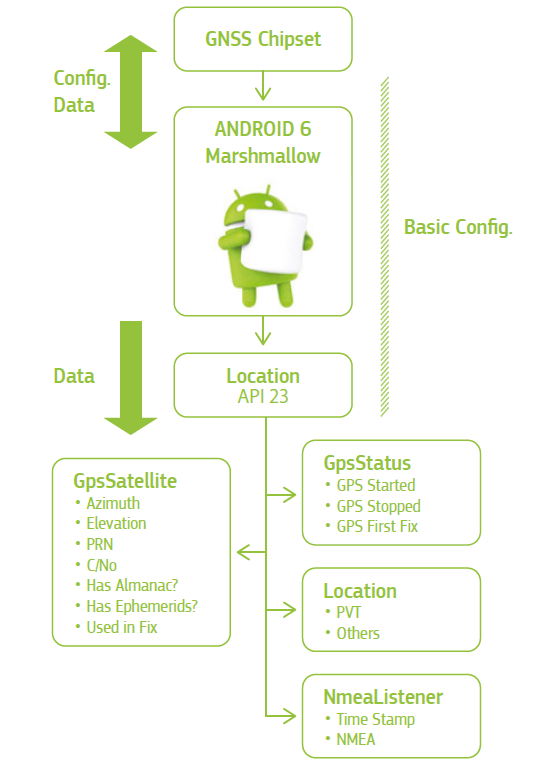
\includegraphics[scale=0.75]{fig/android6API.png} 
	\caption{location API in Android 6}
	\label{FIG:locapiand6} 
\end{figure}

As shown in figure \ref{FIG:locapiand6}, only some basic information computed by the GNSS chipsets were available to the
users. In particular, it was possible to access some GPS satellites information (e.g., C/N\textsubscript{0}, azimuth, and elevation) as well as the basic NMEA (National
Marine Electronics Association) sentences which include
the PVT (Position Velocity and Time) solution. The raw GNSS observations (e.g., pseudorange
and carrier-phase measurements) could not be accessed.  

Starting from the Nougat version (Version 7), Android introduces the new Location API namely \textit{android.location} (figure \ref{FIG:locapiand7}) which gives access to the GNSS raw measurements. However, the new API
implemented on Android 7 does not provide the GNSS measurements directly (e.g., pseudorange, carrier phase and Doppler observations) but the GNSS measurements must be extracted from the raw data logged.
The next paragraphs explain how to obtain GNSS time, pseudoranges,
carrier-phase and Doppler measurements from data contained in \textit{android.location} API. 

\begin{figure}[H] 
	\centering
	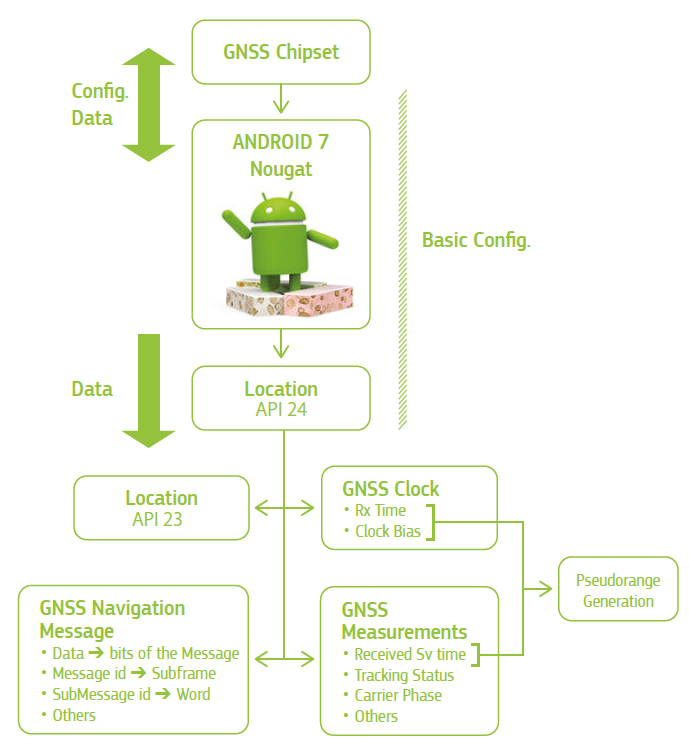
\includegraphics[scale=0.75]{fig/android7API.png} 
	\caption{location API in Android 7}
	\label{FIG:locapiand7} 
\end{figure}

In order to process GNSS measurements from smartphones using common GNSS processing software, as for example RTKLIB \cite{takasu:2009}, the GNSS observation should be derived and written in a standarized format, e.g. RINEX (Receiver INdipendent EXchange format)\footnote{\url{http://acc.igs.org/misc/rinex304.pdf}}. 
Starting from Android 7, GNSS raw observation can be reconstructed by using the informations contained in \textit{Android location API} from level 24 and above see figure \ref{FIG:locapiand7}. The strategy to reconstruct GNSS raw observation is illustrated in \cite{GSA_wp:2016} and hereafter summarized. All the needed information can be retrieved from three classes of \textit{Android location API}:
\clearpage
\begin{itemize}
	{\item GNSS Clock, that contains:}
	\begin{itemize}
		{\item Receiver Time;}
		{\item Clock bias.}
	\end{itemize}
	{\item GNSS Measurement, that contains:}
	\begin{itemize}
		{\item Received Satellite Time;}
		{\item Code;}
		{\item Carrier Phase.}
	\end{itemize}	
	{\item GNSS Navigation Message, that contains:}
	\begin{itemize}
		{\item Navigation Message bits;}
		{\item Navigation Message status.}
	\end{itemize}	
	
\end{itemize}

Table \ref{tab:api_fields} summarizes the most important fields used to reconstruct raw measurements, while table \ref{tab:api_constants} shows the main constants that should be taken into account for the measurement generation, as latter explained.

\begin{table}[H]
	\centering
	\begin{tabular}{|c|c| p{5cm}|}
	\hline
	\textbf{Class} & \textbf{Field} & \textbf{Description}\\
    \hline
	GNSSclock & TimeNanos & GNSS receiver’s internal hardware clock value in nanoseconds\\  
    \hline
	GNSSclock & BiasNanos & Clock’s sub-nanosecond bias\\  
    \hline
	GNSSclock & FullBiasNanos & Difference between TimeNanos inside the	GPS receiver and the true GPS time since 6\textsubscript{th} January 1980\\  
    \hline
	GNSSMeasurement & TimeOffestNanos & Time offset at which the measurement was taken in nanoseconds.\\
    \hline
	GNSSMeasurement & ConstellationType & Constellation type\\  
    \hline
    GNSSMeasurement & Svid & Satellite ID\\  
    \hline
    GNSSMeasurement & State & Per-satellite sync state.	It represents the current	sync state for the associated satellite\\  
    \hline
	GNSSMeasurement & ReceivedTimeNanos & Received GNSS satellite time, at the measurement	time, in nanoseconds\\  
    \hline
	GNSSMeasurement & AccumulatedDeltaRangeMeters & Accumulated delta range since the last channel reset, in meters\\  
    \hline
    GNSSMeasurement & AccumulatedDeltaRangeState & Accumulated Delta Range state\\  \hline
    GNSSMeasurement & CarrierFrequencyHz & Carrier frequency at which codes and messages are modulated\\  
    \hline
    GNSSMeasurement & PseudorangeRatemetersperSecond & Gets the Pseudorange rate at the timestamp\\ 
    \hline
	\end{tabular}
	\caption{Android Location API - Clock and Measurements fields.}
	\label{tab:api_fields}
\end{table}

\begin{table}[H]
	\centering
	\begin{tabular}{| c | c| }
		\hline
		\textbf{Constant} & \textbf{Value (Hexadecimal)}\\
		\hline 
		STATE TOW KNOWN & 0x00004000 \\  
		\hline
		STATE GLO TOD KNOWN & 0x00008000 \\
		\hline
		STATE GAL E1C 2ND CODE LOCK & 0x00008000\\     
		\hline	
	\end{tabular}
	\caption{Android Location API - GNSSMeasurements constants.}
	\label{tab:api_constants}
\end{table}

The quantities retrieved by the proposed program are the pseudorange, the carrier phase, the doppler and C/N\textsubscript{0}. In the following sections, different strategies to compute these quantities are illustrated in details. The methods described were implemented, in the ambit of this work, in a modified version of RTKLIB capable of working with GNSS data from Android (see Appendix \ref{appendix:mrtklib_andr}).
\subsection{Pseudorange computation}  
The equation for the pseudorange is:
\begin{equation}
	\rho = c \cdot (t_{A}-t_{E})
	\label{eq:psrange}
\end{equation}
where \textit{c} is the speed of light, \textit{t\textsubscript{A}} the acquisition time and \textit{t\textsubscript{E}} the emission time of the signal. In the case of smartphones,  \textit{t\textsubscript{A}} and  \textit{t\textsubscript{E}} are calculated considering the \textit{GNSS Clock} class (used for receiver-related quantities) and the  \textit{GNSS Measurement} class. 
The receiver time is generated considering the TimeNanos quantity, which is the GNSS receiver’s internal hardware clock provided as an integer number of nanoseconds. The FullBiasNanos quantity, i.e., the difference between the TimeNanos inside the GPS receiver and the true GPS time since the 6\textsuperscript{th} of January 1980 must be subtracted to the TimeNanos in order to get the true GPS time. So the receiver time can be written as:

\begin{equation}
	T_{Rx} = TimeNanos - FullBiasNanos
	\label{eq:Trx_int}
\end{equation}

The API also provides the BiasNanos quantity, i.e. the clock’s sub-nanosecond bias (varying between 0 and 1), which allows getting a more accurate timing. Considering also the BiasNanos, the receiver time becomes:

\begin{equation}
	T_{Rx} = TimeNanos - (FullBiasNanos + BiasNanos)
	\label{eq:Trx_flt}
\end{equation}
Both the GNSS RawMeasurements Task Force \cite{GSA_wp:2016} and Google in its GNSS analysis tool available online suggest considering only the first value of the FullBiasNanos and BiasNanos and keep them constant for all the acquisition. In this work, as suggested in \cite{darugna2021}, FullBiasNanos and BiasNanos are updated every epoch. Indeed, in \cite{darugna2021} the authors observe that, depending on the device firmware, FullBiasNanos values can have significant oscillations, hence they cannot be considered as constant.


The received satellite time, i.e. ReceivedSvTimeNanos, is relative to the beginning of the system week for all constellations except for GLONASS, where it is relative to the beginning of the GLONASS system day. Therefore, depending on the GNSS involved, the condition of
reliability of the received satellite time is satisfied if:

\begin{itemize}
	{\item  GPS, Galileo, and BeiDou: STATE TOW KNOWN constant flag is set}
	{\item  GLONASS: STATE GLO TOD KNOWN constant flag is set}
\end{itemize}

The constant values of STATE TOW KNOWN and STATE GLO TOD KNOWN are reported in table \ref{tab:api_constants}.

These flags provide an insight into the state of the tracking algorithms that must be taken into account to verify the reliability of the measurement. It’s worth mentioning that some devices track the Galileo E1C component, and the tracking status is flagged as the STATE GAL E1C 2ND CODE LOCK (see table \ref{tab:api_constants}). In this case, the ambiguity of the pseudorange is 100ms, another parameter to take into account.

The satellite emission time can be than computed as:

\begin{equation}
	T_{E,TOW} = ReceivedTimeNanos
	\label{eq:Te_tow}
\end{equation}
 
in GPS Time Of theWeek (TOW) for GPS, Beidou and Galileo, and

\begin{equation}
	T_{E,TOW} = ReceivedTimeNanos
	\label{eq:Te_tod}
\end{equation}

in GPS Time Of the Day (TOD) for GLONASS.

Once the receiver and satellite time have been computed, the pseudorange observation can be reconstructed. Receiver and satellite time as computed in eq \ref{eq:Trx_flt} and eq \ref{eq:Te_tow} (or eq \ref{eq:Te_tod}) are expressed in GPS time and GPS TOW/TOD, respectively. To solve this data type inconsistency, two possible options are possible:

\begin{itemize}
	\item to compute the receiver time in GPS TOW;
	\item to compute the satellite time in GPS time.
\end{itemize}

In the first case the receiver time can be computed in the following ways.

For GPS and Galielo:

\begin{equation}
	T_{Rx} = mod(T_{Rx,GT},NanoSecondsWeek)
	\label{eq:Trx_gps_gal_tow}
\end{equation}

For Beidou:

\begin{equation}
	T_{Rx} = mod(T_{Rx,GT},NanoSecondsWeek) + 14\cdot10^{9}
	\label{eq:Trx_beid_tow}
\end{equation}

And for GLONASS:

\begin{equation}
	T_{Rx} = mod(T_{Rx,GT},NanoSecondsDay) + (7200-ls)\cdot10^{9}
	\label{eq:Trx_glo_tow}
\end{equation}

Where \textit{NanoSecondsWeek} is the number of nanoseconds in a week, and \textit{NanoSecondsDay} and \textit{ls} (see eq \ref{eq:Trx_glo_tow}) are the nanoseconds in a day and the leap seconds respectively.

In the latter case, i.e., when computing satellite time in GPS time, the equation for GPS and Galileo becomes:

\begin{equation}
	T_{E} = T_{E,TOW} + nw\cdot NanoSecondsWeek
	\label{eq:Te_gps_gal_gpstime}
\end{equation}

While the equantion for BeiDou is:

\begin{equation}
	T_{E} =  T_{E,TOW} + nw\cdot NanoSecondsWeek +  14\cdot10^{9}
	\label{eq:Te_beidou_gpstime}
\end{equation}

And for GLONASS:

\begin{equation}
	T_{E} =  T_{E,TOD} + NanoSecondsDaySince1980 +  (7200-ls)\cdot10^{9} 
	\label{eq:Te_glo_gpstime}
\end{equation}

Where \textit{nw} (see equations \ref{eq:Te_gps_gal_gpstime} and \ref{eq:Te_beidou_gpstime}) is the number of weeks since 6\textsuperscript{th} January 1980, and \textit{NanoSecondsDaySince1980} is the days since 6\textsuperscript{th} January 1980 in nanoseconds.

Lastly, for each observation, the time offset at which the measurement was taken with regard to the TimeNanos has to be considered: this quantity is given by TimeOffsetNanos. The acquisition time  becomes then:

\begin{equation}
	T_{A} =  T_{Rx} + TimeOffsetNanos
	\label{eq:Ta_android}
\end{equation}

Finally, the pseudorange observation can be computed in meters in the followig way:

\begin{equation}
	\rho = \frac{ c \cdot (T_{Rx}-T_{E})}{10^{9}}
	\label{eq:pseudorange_android}
\end{equation}

\subsection{Carrier Phase observation computation}

Carrier phase measurements are provided directly by API the  as \textit{AccumulatedDeltaRangeMeters} in metres. Often in GNSS standard format the phase measurement are expressed in number of cycles and not in meters. In order to express the phase measurement in cycles, the \textit{AccumulatedDeltaRangeMeters} should be divided by the wavelength.

\begin{equation}
	\phi = \frac{AccumulatedDeltaRangeMeters}{\lambda}
	\label{eq:phase_cycles}
\end{equation}

The $\lambda$ value can be obtained from the API, by dividing the field \textit{CarrierFrequencyHz} by the speed of light.
 
Carrier phase observation are ambiguous, without the time information, meaning the receiver can only count the number of cycles occurring between epochs (as explained in riferimento capitolo1), and, for example if a cycle slip occurs, the receiver loses this count. For this and also other reasons the \textit{AccumulatedDeltaRangeMeters} field is paired with the \textit{AccumulatedDeltaRangeState}. The \textit{AccumulatedDeltaRangeState}, which values are reported in table \ref{tab:adr_state}, it's possibile to check the validity status of the carrier phase observation.

\begin{table}[h]
	\centering

	\begin{tabular}{| c | c| c|}
		\hline
		\textbf{Status} & \textbf{Value} & \textbf{Description)}\\
		\hline 
		ADR STATE CYCLE SLIP & 4 & A cycle slip has been detected.\\
		\hline
		ADR STATE RESET & 2 & A reset has been detected.\\
		\hline
		ADR STATE VALID & 1 & State is valid.\\     
		\hline	
		ADR STATE UNKNOWN & 0 & State is unknown.\\     
		\hline
	\end{tabular}
\caption{Accumulated delta range state valued}
\label{tab:adr_state}
\end{table}

Concerning carrier phase observation on smartphones, it is worth mentioning the potential problems related to duty cycle. The duty cycle is a process where the GNSS chipset of the smartphone works in a discontinuous way, which causes the hardware clock to be active only for a fraction of each second to support low power consumption and, thus, reduce battery consumption. \cite{Linty:2014}. 

\begin{figure}[htb] 
	\centering
	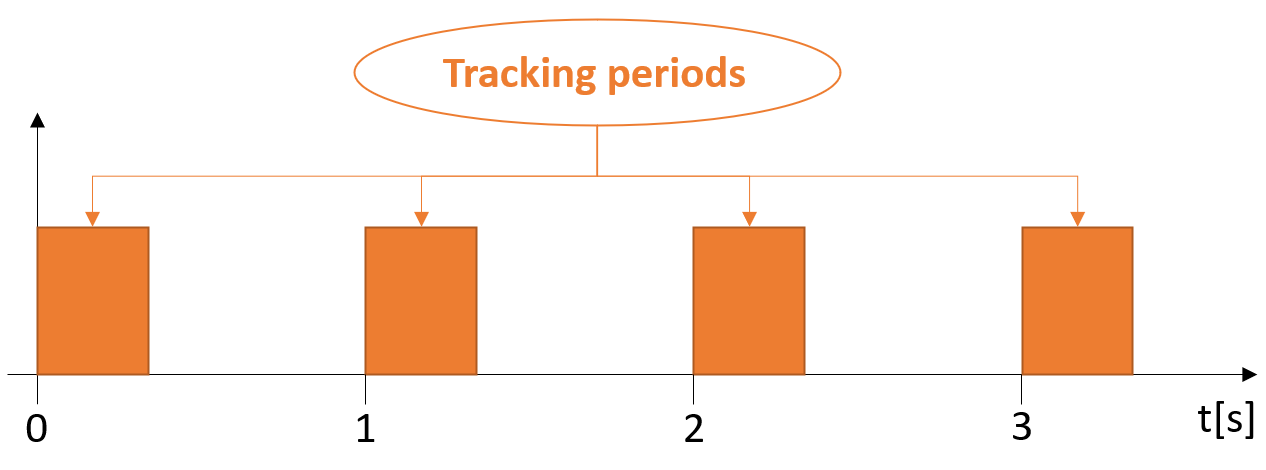
\includegraphics[scale=0.60]{fig/duty_cycle.png} 
	\caption{Duty cycle versus time}
	\label{FIG:duty_cycle} 
\end{figure}
As explained in \cite{GSA_wp:2016}, there are two different implementations of the duty-cycle that depend on the GNSS clock status:
\begin{itemize}
	\item TCXO Hardware clock is not continuous (turning on and off) during the non-tracking periods;
	\item TCXO Hardware clock is continuous during the non-tracking periods.
\end{itemize}
The smartphone has two oscillators: higher precision compensated for temperature variations (TCXO) that is being used for GNSS tracking and an alternative, low-power consumption, crystal oscillator (XO). In the first case, during the short tracking period, when the chipset tracks GNSS data, TCXO is used. 
Out of this period, when a chip shuts down for several hundreds of milliseconds, XO is providing time. In the latter case, when the GNSS chipset is turned off, the TCXO clock keeps running, even though no signal is being tracked. 
Users cannot detect when the receivers are operating in
duty cycle. Without going in further details, which is not the purpose of this work, it should be clear that duty cycle has
an impact on the carrier phase measurements. Indeed, without tracking continuity, several cycle slips may occur between two
consecutive measurements, severely limiting the use of  advance phase techniques such as Real Time Kinematic.

Starting from Android 9, it has been introduced an option to disable the duty cycle. Thanks to this option, it's possible to use GNSS carrier phase observation from smartphone.

\subsection{Doppler computation}
 The Doppler shift that results from satellite movement can be derived from the \textit{PseudorangeRateMetersPerSecond}, provided
 that the pseudorange rate, at the timestamp, is in m/s. In particular it's given by:
 
 \begin{equation}
 	Dopplershift = -\frac{PseudorangeRateMetersPerSecond}{\lambda}  	\label{eq:doppler_and}
 \end{equation}

Where $\lambda$ is the wavelength.

Once the GNSS raw observable are reconstructed they can be processed by common GNSS processing software in order to retrieve the position following the principles illustrated in chapter \ref{ch:gnss}. 


In this thesis work, the software library used for all experiments are based on RTKLIB. This software is widely use from the scientific community for research purposes on GNSS.
It implements different positioning methods and, being open source, it can be easily modified and adapted to specific cases. As latter explained, in the ambit of this work, the RTKLIB software library has been modified in order both to work in real time with data coming from Android smartphones and to implement an algorithm for increasing the positioning robustness. In the following paragraph the RTKLIB software is illustrated in details, with particular attention to the algorithms that i natively implements for GNSS positioning.

\section{RTKLIB for data processing}
RTKLIB \cite{takasu:2009}  is an open source portable program library written in C and C++ which provides a platform for precise GNSS positioning. The current version of the library is distributed under the following BSD 2-clause license and additional exclusive clauses. Previous versions of RTKLIB until ver. 2.4.1 had been distributed under GPLv3 license.
The quite satisfactory performance of the library and  specific characteristics of the licence, which allows free exploitation for commercial applications made RTKLIB, made it very popular and extensively exploited. 
\subsection{Software description}
The library implements fundamental navigation functions and carrier-based relative positioning algorithms both in real time as well as in post processing. In spite of its name, however, it is not limited to RTK relative positioning but implement also many other stand alone and relative positioning techniques, like Single, DGPS/DGNSS, Kinematic, Static, Moving-Baseline, Fixed, PPP-Kinematic, PPP-Static and PPP-Fixed.
RTKLIB is able to estimate integer ambiguity exploiting the LAMBDA method \cite{Teunissen_ar1995} . 
RTKLIB was originally developed under the Windows Operating System, and later it has been ported under UNIX environment which allows to use it in small and compact single-board computer, as for example, the Raspberry integrated into the PID. 
RTKLIB is a GNSS processing software since, in addition to GPS, it supports also GLONASS, GALILEO, QZSS, BeiDou and SBAS.
Moreover it supports many standard formats and protocols for GNSS: 
\begin{itemize}
\item RINEX 2.10, 2.11, 2.12 OBS/NAV/GNAV/HNAV/LNAV/QNAV,
\item RINEX 3.00, 3.01 OBS/NAV,
\item RINEX 3.02 OBS/NAV/CLK,
\item RTCM 2.3, 3.1(with amendment 1-5), 3.2,
\item BINEX,
\item NTRIP 1.0,
\item RTCA/DO-229C,
\item NMEA 0183,
\item SP3-c,
\item ANTEX 1.4,
\item IONEX 1.0, 
\item NGS PCV and EMS 2.0.
\end{itemize}

RTCM (Radio Technical Commission for Maritime Services) standar in particular, is a communication protocol for sending differential corrections to a GNSS receiver from a secondary source. The format does not define the source of the messages and has been used with systems as varied as longwave marine radio, communications satellite broadcasts, and internet distribution. NTRIP (Networked Transport of RTCM via Internet Protocol) instead is an application-level protocol that
supports streaming GNSS data over the Internet. which is meant to be an open non-proprietary protocol.

RTKLIB supports also several GNSS receivers' proprietary messages like NovAtel, OEM4/V/6, OEM3, OEMStar, Hemisphere, u-blox, JAVAD and other. 
It also supports external communication via: Serial port, TCP/IP, NTRIP, local log file (record and playback) and FTP/HTTP (automatic download).
The library include a full set of functions suitable to be exploited both for geodesy or precise navigation application and the processing is configurable to optimize the retrieved solution. 
Among the different function it's worth mentioning: 
\begin{itemize}
\item matrix and vector computation functions,
\item time and string functions,
\item coordinates transformation, 
\item input and output functions,
\item debug trace functions, platform dependent functions, 
\item positioning models, 
\item atmosphere, antenna, earth tides ocean loading models, 
\item geoid models and  datum transformation, 
\item precise ephemeris and satellite clock handling functions, 
\item Google Earth KML converter, 
\item SBAS functions, 
\item integer ambiguity resolution, 
\item standard positioning, real time precise positioning and post-processing positioning, 
\item stream and  RTK server functions, 
\item downloader functions
\end{itemize}
Going into details, RTKLIB provides APIs for real-time positioning, post-processing analysis, and positioning utilities. Table \ref{tab:rtklib_apps} shows the main RTKLIB APPs in their GUI (Graphical User Interface) version and CUI (Command-line User Interface) version. In the ambi of this work the CUI APs are used and in particular RTKRCV for computing the Real-Time Positioning.
\begin{table}[ht]
	\centering
	\begin{tabular}{| c | c| c|}
		\hline
		\textbf{Function} & \textbf{GUI App} & \textbf{CUI App}\\
		\hline 
		App launcher & RTKLAUNCH  & -\\
		\hline
		Real time positioning & RTKNAVI & RTKRCV\\
		\hline
		Communication Server & STRSVR & STR2STR\\     
		\hline	
		Post processing analysis & RTKPOST & RNX2RTKP\\     
		\hline
		RINEX Converter & RTKCONV & CONVBIN\\     
		\hline
		Plot solutions and observation data & RTKPLOT & -\\     
		\hline
		Download GNSS data and products & RTKGET & -\\     
		\hline
	\end{tabular}
\caption{RTKLIB Apps}
\label{tab:rtklib_apps}
\end{table}
\subsection{Software computation strategy}
RTKLIB, as well explained in \cite{takasu:2009}, uses algorithms for differential GNSS positioning. In particular, for carrier-based relative
positioning with a short length baseline between rover \textit{a} and
base-station \textit{b}, the equation \ref{eq:triple_diff0} is used. This equation can be also written as
\begin{equation} 
	\begin{matrix} 
		{\Phi_{ab}}^{ij}={\rho_{ab}}^{ij}+\lambda(B_{ab}^{i}-B_{ab}^{j})+ \textit{d}\Phi_{a}^{S}+\epsilon_{\Phi}\\ 
		{P_{ab}}^{ij}={\rho_{ab}}^{ij}+  \epsilon_{P}
		\end{matrix}
	\\
	\label{eq:ddiff_rtklib}
\end{equation}

where $\rho$ is the geometric range, $\lambda$ is the carrier wave length and $\epsilon$ is the measurement error of 
these observables, $B_{ab}^{i}$ is single-difference of carrier-phase ambiguities in cycle, and $\textit{d}\Phi_{a}^{S}$ is the carrier‐phase correction terms, which can be neglected in the short‐baseline case.
Thanks to the double differencing procedure, equations are free of satellite and receiver clock-biases, and
atmospheric effects, as explained in chapter \ref{ch:gnss}.
After computing these equations, a vector \textbf{\textit{x}} containing the unknown state for RTK-GPS positioning is set:

\begin{equation} 
	\begin{matrix} 
		{\textbf{\textit{x}}}=({\textbf{\textit{r}}_{a}}^{T}+{\textbf{\textit{B}}_{L1}}^{T}+{\textbf{\textit{B}}_{L2}}^{T} + +{\textbf{\textit{B}}_{L5}}^{T})^{T}\\ 
		\textbf{\textit{B}}_{Lj}=({{B}_{Lj}}^{1}, {{B}_{Lj}}^{2},...,{{B}_{Lj}}^{m})^{T}
		\end{matrix}
	\\
	\label{eq:unkstate_rtklib}
\end{equation}
where $\textbf{\textit{r}}_{a}$ is rover antenna position in ECEF frame, and $m$ is the number of satellites used. The measurement vector ${\textbf{\textit{y}}}_{k}$ at the epoch $\textit{t}_{k}$ is
defined with double-differenced carrier-phase and pseudorange
measurements as:

\begin{equation} 
	\begin{matrix} 
		\textbf{y}_{k}= ({\boldsymbol{\Phi}_{L1}}^{T}, {\boldsymbol{\Phi}_{L2}}^{T},{\boldsymbol{\Phi}_{L5}}^{T}, {\textbf{P}_{L1}}^{T},{\textbf{P}_{L2}}^{T}, {\textbf{P}_{L5}}^{T})^{T}\\ 
		\boldsymbol{\Phi}_{Lj}= ({\Phi_{ab,lj}}^{12},{\Phi_{ab,lj}}^{13},...,{\Phi_{ab,lj}}^{1m})^{T}\\
        \textbf{P}_{Lj}= ({P_{ab,lj}}^{12},{P_{ab,lj}}^{13},...,{P_{ab,lj}}^{1m})^{T}\\
		\end{matrix}
	\\
	\label{eq:measvector_rtklib}
\end{equation}

RTKLIB estimates the state vector
\textbf{\textit{x}} and its covariance matrix \textbf{\textit{P}} using a standard EKF Extended Kalman Filter \cite{kalman:1960, grewal2001}. The used equations are:

\begin{equation} 
	\begin{matrix} 
		\hat{\textbf{\textit{x}}_{k}}(+)= \hat{\textbf{\textit{x}}_{k}}(-) + \textbf{\textit{K}}_{k}\cdot \left[ \textbf{\textit{y}}_{k}-\textbf{\textit{h}}\left(\hat{\textbf{\textit{x}}_{k}}(-)\right) \right]\\ 
		\textbf{\textit{P}}_{k}(+)= \left(\textbf{\textit{I}}-\textbf{\textit{K}}_{k} \textbf{\textit{H}}_{k}\left(\hat{\textbf{\textit{x}}_{k}}(-) \right)\right) \left( \textbf{\textit{P}}_{k}(-)\right)\\
		\textbf{\textit{K}}_{k}= \textbf{\textit{P}}_{k}(-)\textbf{\textit{H}} \left( \hat{\textbf{\textit{x}}_{k}}(-) \right) \left( \textbf{\textit{H}} \left( \hat{\textbf{\textit{x}}_{k}}(-) \right) \textbf{\textit{P}}_{k}(-) \textbf{\textit{H}} \left( \hat{\textbf{\textit{x}}_{k}}(-) \right)^{T} + \textbf{\textit{R}}_{k} \right)^{-1}
		\end{matrix}
	\\
	\label{eq:EKF_rtklib}
\end{equation}
Where $\textbf{\textit{h(x)}}$, $\textbf{\textit{H(x)}}$ and \textbf{\textit{R\textsubscript{k}}} are the measurements model vector, the
matrix of partial derivatives and the covariance matrix of
measurement errors, respectively. Considering equations \ref{eq:ddiff_rtklib} they can be written as:
\begin{equation} 
	\begin{matrix} 
		\textbf{\textit{h}}(\hat{\textbf{\textit{x}}})= \left( {\textbf{\textit{h}}_{\Phi,L1}}^{T}, {\textbf{\textit{h}}_{\Phi,L2}}^{T},  {\textbf{\textit{h}}_{\Phi,L5}}^{T}, {\textbf{\textit{h}}_{P,L1}}^{T}, {\textbf{\textit{h}}_{P,L2}}^{T}, {\textbf{\textit{h}}_{P,L5}}^{T}\right)\\
		\textbf{\textit{h}}_{\Phi,Lj} = \begin{bmatrix} 
                {\rho_{ab}}^{12} + \lambda_{Lj} \left( B_{ab,Lj}^{1} - B_{ab,Lj}^{2} \right)  \\
                {\rho_{ab}}^{13} + \lambda_{Lj} \left( B_{ab,Lj}^{1} - B_{ab,Lj}^{3} \right)  \\
                \vdots\\
               {\rho_{ab}}^{1m} + \lambda_{Lj} \left( B_{ab,Lj}^{1} - B_{ab,Lj}^{m} \right)  \\ \\
                \end{bmatrix}, & \textbf{\textit{h}}_{P,Lj} = \begin{bmatrix} 
                {\rho_{ab}}^{12}  \\
                {\rho_{ab}}^{13}  \\
                \vdots\\
               {\rho_{ab}}^{1m}  \\
                \end{bmatrix} 
        
		\end{matrix} \\
	\label{eq:EKF_rtklib_h}
\end{equation}

\begin{equation}
	\textbf{\textit{H}}(\hat{\textbf{\textit{x}}}) = \frac{\partial \textbf{\textit{h}}(\hat{\textbf{\textit{x}}})}{\partial \textbf{x}} \bigg|_{x=\hat{x}} = \begin{bmatrix}
	    \textbf{\textit{-DE}} & 0 & \lambda_{L1}\textbf{\textit{D}} &0&0\\
	    \textbf{\textit{-DE}} & 0 & 0 &\lambda_{L2}\textbf{\textit{D}}&0\\
	    \textbf{\textit{-DE}} & 0 & 0 &0&\lambda_{L5}\textbf{\textit{D}}\\
	    \textbf{\textit{-DE}} & 0 & 0 &0&0\\
	    \textbf{\textit{-DE}} & 0 & 0 &0&0\\
	    \textbf{\textit{-DE}} & 0 & 0 &0&0\\
	\end{bmatrix}
	\label{eq:EKF_rtklib_H}
\end{equation}

\begin{equation}
\begin{matrix}
\textbf{\textit{R}}_{k} = \begin{bmatrix}
\textbf{\textit{D}}\textbf{\textit{R}}_{\Phi,L1}{\textbf{\textit{D}}}^{T} &&&&&\\
&\textbf{\textit{D}}\textbf{\textit{R}}_{\Phi,L2}{\textbf{\textit{D}}}^{T}&&&&\\
&&\textbf{\textit{D}}\textbf{\textit{R}}_{\Phi,L5}{\textbf{\textit{D}}}^{T}&&&\\
&&&\textbf{\textit{D}}\textbf{\textit{R}}_{P,L1}{\textbf{\textit{D}}}^{T}&&\\
&&&&\textbf{\textit{D}}\textbf{\textit{R}}_{P,L2}{\textbf{\textit{D}}}^{T}&\\
&&&&&\textbf{\textit{D}}\textbf{\textit{R}}_{P,L5}{\textbf{\textit{D}}}^{T}\\
\end{bmatrix}\\
{\rho_{a}}^{i}=\| \hat{\textbf{\textit{r}}}_{a} - \textbf{\textit{r}}^{j} \|,  {\rho_{b}}^{i}= \|\textbf{\textit{r}}_{b} - \textbf{\textit{r}}^{j}\|,  \textbf{\textit{E}}= \left({\textbf{\textit{e}}_{a}}^{1^{T}},{\textbf{\textit{e}}_{a}}^{2^{T}},...,{\textbf{\textit{e}}_{a}}^{m^{T}}  \right)^{T}\\
\textbf{\textit{R}}_{\Phi,Lj}= 2diag \left( {\sigma_{\Phi,Lj}^{1}}^{2}, {\sigma_{\Phi,Lj}^{2}}^{2},...,{\sigma_{\Phi,L1}^{m}}^{2}\right)\\
\textbf{\textit{R}}_{P,Lj}= 2diag \left( {\sigma_{P,Lj}^{1}}^{2}, {\sigma_{P,Lj}^{2}}^{2},...,{\sigma_{P,L1}^{m}}^{2}\right)\\

\textbf{\textit{D}}= \begin{bmatrix}
1&-1&0&\dots&0\\
1&0&-1&\dots&0\\
\vdots&\vdots&\vdots&\ddots&\vdots\\
1&0&0&\dots&-1\\
\end{bmatrix}

\end{matrix}
\\
\label{eq:EKF_rtklib_Rk}
\end{equation}

Where \textbf{\textit{r}}\textsuperscript{i} is satellite \textit{i} position in ECEF frame, \textbf{\textit{r}}\textsubscript{b} is base station antenna position, \textbf{\textit{e}}\textsubscript{a}\textsuperscript{i} is line-of-sight vector from rover
antenna to satellite \textit{i}, \textbf{\textit{D}} is single-differencing matrix, and $\sigma_{\Phi}$ and $\sigma_{P}$ are standard deviation of phase‐range measurement error and the standard deviation of pseudorange measurement error respectively.  For the standard deviation $\sigma$ of carrier-phase or pseudorange error, RTKLIB employs a priori elevation-dependent model with user-defined parameters. 
The time update of the state vector and its covariance matrix from epoch \textit{t}\textsubscript{k} to epoch \textit{t}\textsubscript{k+1} by EKF is expressed as:

\begin{equation}
\begin{matrix}
    \hat{\textbf{\textit{x}}}_{k+1}(-) = \textbf{\textit{F}}_{k}^{k+1} \hat{\textbf{\textit{x}}}_{k}(+)\\
    \textbf{\textit{P}}_{k+1}(-)=\textbf{\textit{F}}_{k}^{k+1}\textbf{\textit{P}}_{k}(+) \textbf{\textit{F}}_{k}^{{k+1}^{T}} + \textbf{\textit{Q}}_{k}^{k+1}\\
\end{matrix}
\\
\label{eq:EKF_rtklib_tupdate}
\end{equation}

where \textbf{\textit{F}} is the state transition matrix and \textbf{\textit{Q}} is the covariance matrix of system noise. 
In the kinematic positioning mode, a white noise model should be assumed for the rover antenna position as:

\begin{equation}
    \begin{matrix}
        \textbf{\textit{F}}_{k}^{k+1}=\begin{bmatrix}
        \textbf{\textit{I}}_{3x3} & & \\
        & \textbf{\textit{I}} & \\
        & & \textbf{\textit{I}}_{(3\textit{m}-3) x(3\textit{m}-3)}\\
        \end{bmatrix}, & \textbf{\textit{Q}}_{k}^{k+1} =\begin{bmatrix}
        \infty_{3x3} & & \\
        &  \textbf{\textit{0}}_{3x3} & \\
        & &  \textbf{\textit{0}}_{(3\textit{m}-3) x(3\textit{m}-3)}\\
        \end{bmatrix}
    \end{matrix}
\\
\label{eq:EKF_rtklib_FQ}
\end{equation}

where the carrier-phase ambiguities are assumed to be stationary. To avoid numerical instability by adding infinite process noises to the variances of the receiver position, the receiver position states are instead reset to the initial guess values at every epochs and adequately large process noises (10\textsubscript{4} m\textsubscript{2}) are added to the variance in RTKLIB. The initial position is derived from
the single point positioning process which is used to avoid the iteration for non‐linear signal
measurement model. In the static positioning mode, RTKLIB uses just a
simple state transition model defined as \textbf{\textit{F}} = \textbf{\textit{I}} and \textbf{\textit{Q}} = \textbf{\textit{0}}. Regarding to
the single-differenced carrier-phase ambiguity terms, the initial
states are determined as the guess estimated values by
carrier-phase minus pseudorange. If a cycle-slip is detected, the
state of the carrier-phase ambiguity is reset to initial state in the
same manner. To detect cycle-slips, RTKLIB monitors the jump
of the geometry-free LC (linear combination) of L1 and L2
carrier-phase as well as LLI (loss of lock indicator) and lock-time
provided by the receiver.

By solving the EKF formulas (see eq. \ref{eq:EKF_rtklib} with the RTK GPS equations
described above (eq \ref{eq:ddiff_rtklib}), the estimated rover antenna position and the
single-differenced carrier-phase ambiguities are obtained. The
estimated rover antenna position is frequently referred to as
"FLOAT" solution without integer ambiguity resolution.

Once the estimated states obtained, the float carrier-phase
ambiguities should be resolved into integer values in order to
improve accuracy and convergence time. In RTKLIB, the float
solution of the rover position and the single-differenced
carrier-phase ambiguities are transformed to double-differenced
forms by:

\begin{equation}
    \begin{matrix}
        \hat{\textbf{\textit{x}}}_{k}^{'}= \textbf{\textit{G}}  \hat{\textbf{\textit{x}}}_{k} (+) = \left({\hat{\textbf{\textit{x}}}_{k}}^{T} {\hat{\textbf{\textit{N}}}}^{T}\right)^{T}
        \\

    \textbf{\textit{P}}_{k}^{'}=\textbf{\textit{G}} \textbf{\textit{P}}_{k}(+) \textbf{\textit{G}}^{T}= \begin{bmatrix}
    \textbf{\textit{Q}}_{R} & \textbf{\textit{Q}}_{NR}\\
    \textbf{\textit{Q}}_{NR} & \textbf{\textit{Q}}_{N}\\
    \end{bmatrix}
\\
\textbf{\textit{G}}=\begin{bmatrix}
\textbf{\textit{I}}_{3}&&\\
&\textbf{\textit{D}}&\\
&&\textbf{\textit{D}}\\
\end{bmatrix}
\end{matrix}
\\
\label{eq:rtklib_cp_ddidd}
\end{equation}

where \textbf{\textit{N}} is the double differenced carrier-phase ambiguities,
which should be integers by canceling the receiver initial phase
terms. In this form, the best integer vector $\tilde{\textbf{\textit{N}}}$
is searched to satisfy the condition of Integer Least Square (ILS) problem as:
\begin{equation}
\tilde{\textbf{\textit{N}}}=  \argmin_{N \epsilon \textbf{\textit{Z}}} \left( \left( \textbf{\textit{N}} - \hat{\textbf{\textit{N}}} \right)^{T} {\textbf{\textit{Q}}_{N}}^{-1} \left( \textbf{\textit{N}} - \hat{\textbf{\textit{N}}} \right) \right)
\label{eq:interger_amb_ILS_N}    
\end{equation}

To solve the problem, RTKLIB exploits the well-known efficient strategy LAMBDA \cite{Teunissen_ar1995} and its extension MLAMBDA \cite{chang2005}. LAMBDA and MLAMBDA offer the combination of a linear
transformation to shrink the integer vector search space and a skillful tree‐search procedure in the
transformed space. The integer vector solution by these procedures is validated by the following
simple \textit{Ratio‐Test}. In the \textit{Ratio‐Test} (eq \ref{eq:rtklib_ratiotest}), the ratio‐factor \textit{R}, defined as the ratio of the weighted sum of the squared residuals by the second best solution $\tilde{\textbf{\textit{N}}}_{2}$ to one by the best $\tilde{\textbf{\textit{N}}}$, is used to check the reliability of the solution.
\begin{equation}
\textit{R}=\frac{\left( \tilde{\textbf{\textit{N}}}_{2} - \hat{\textbf{\textit{N}}} \right)^{T} {\textbf{\textit{Q}}_{N}}^{-1} \left( \tilde{\textbf{\textit{N}}}_{2} - \hat{\textbf{\textit{N}}} \right) }{\left( \tilde{\textbf{\textit{N}}} - \hat{\textbf{\textit{N}}} \right)^{T} {\textbf{\textit{Q}}_{N}}^{-1} \left( \tilde{\textbf{\textit{N}}} - \hat{\textbf{\textit{N}}} \right)} > \textit{R}_{thres}
\label{eq:rtklib_ratiotest}
\end{equation}

The validation threshold \textit{R}\textsubscript{\textit{Rthres}}, in eq \ref{eq:rtklib_ratiotest} can be set by the user in the processing option  \textit{"Min Ratio to Fix Ambiguity"}. 

After the validation, the  "FIXED" solution of the rover antenna position $\tilde{\textbf{\textit{r}}}_{a}$ is obtained by solving the following equation. 

\begin{equation}
\tilde{\textbf{\textit{r}}}_{a}=\hat{\textbf{\textit{r}}}_{a}- \textbf{\textit{Q}}_{RN}-{\textbf{\textit{Q}}_{N}}^{-1} \left(\hat{\textbf{\textit{N}}} -\tilde{\textbf{\textit{N}}}\right)
\label{eq:rtklib_solution}
\end{equation}

If the validation failed, the solution is considered  "FLOAT" and RTKLIB returns $\hat{\textbf{\textit{r}}}_{a}$ instead of $\tilde{\textbf{\textit{r}}}_{a}$.
